\section{Diagrama Entidad-Relación}

Para que sea más sencillo entender nuestro modelo, iremos presentando las diferentes partes del DER en secciones y explicando cómo resolvemos los diferentes problemas. Analizaremos las entidades y relaciones más complejas, que consideramos son vitales al sistema. Las demás se podrán ver en el DER completo.\\

\subsection{Personas}
\begin{figure}[H]
   \begin{center}
   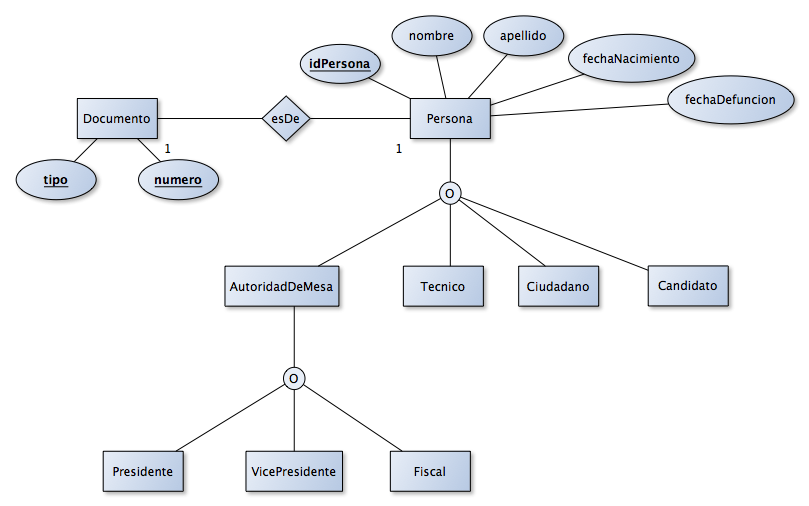
\includegraphics[scale=0.5]{graphics/der_personas.png}
   \caption{\textbf{Personas}}
   \label{fig:der}
   \end{center}
\end{figure}

Para facilitar la relación de las personas con las diferentes entidades del sistema decidimos dividir a las Personas según los roles que ocupan.\\

Es importante notar que cada herencia es \textit{overlapping}, para poder modelar que una persona que es Autoridad de Mesa en una elección, puede ser Candidato en la siguiente, por ejemplo.\\

Esto significa que cada rol guarda una tupla con el \textit{idPersona} si dicha Persona cumplió alguna vez con ese rol.\\

Notemos también que decidimos mantener una clave artificial, \textit{idPersona}, como identificador dentro del sistema para facilitar el movimiento de esta clave como clave foránea, en lugar de \textit{número} y \textit{tipo} de Documento.\\

\subsection{Territorios}
\begin{figure}[H]
   \begin{center}
   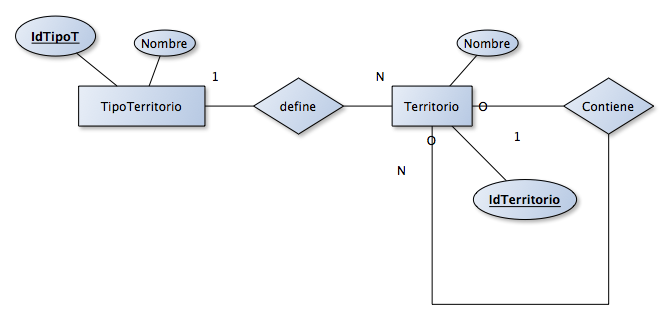
\includegraphics[scale=0.5]{graphics/der_territorios.png}
   \caption{\textbf{Territorios}}
   \label{fig:der}
   \end{center}
\end{figure}

Entendiendo que nuestro sistema debe soportar elecciones para diferentes partes del país, a diferentes niveles, decidimos modelar los Territorios en una jerarquía recursiva. Cada territorio puede contener otros territorios, y a su vez, cada territorio puede ser contenido por otro.\\

Los tipos de territorios disponibles que consideramos apropiados son:
\begin{itemize}
	\item{País}
	\item{Provincia}
	\item{Localidad}
	\item{Ciudad}
\end{itemize}

De esta manera consideramos que un País contiene Provincias, que contiene Localidades o Ciudades. Formalmente, las restricciones asociadas son:
\begin{itemize}
	\item{Un País sólo puede contener Provincias.}
	\item{Una Provincia sólo puede contener Localidades o Ciudades.}
	\item{Una Localidad sólo puede contener Ciudades.}
	\item{Una Ciudad no puede contener nada.}
\end{itemize}

\subsection{Mesas electorales}
\begin{figure}[H]
   \begin{center}
   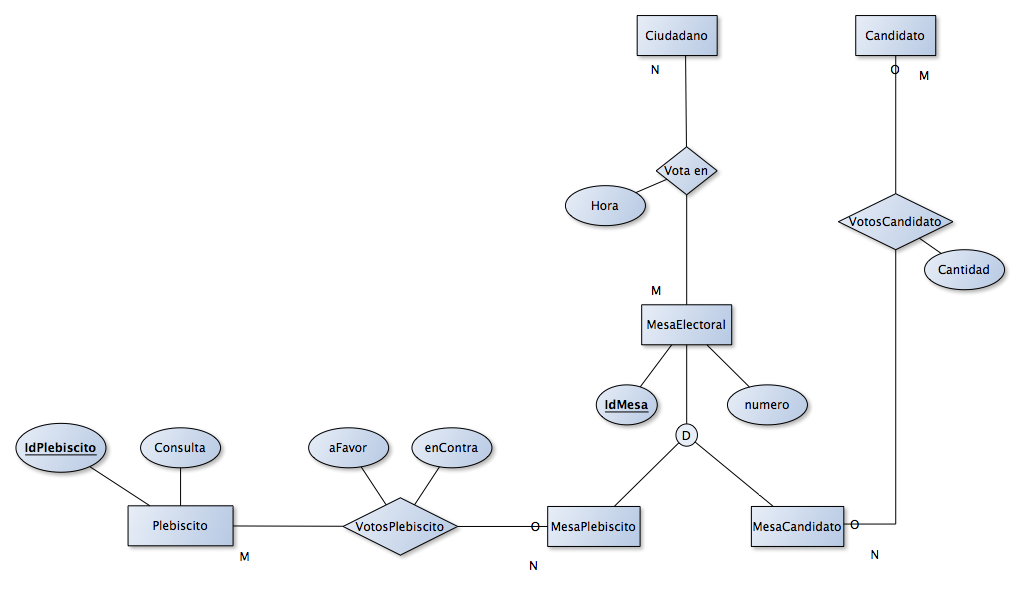
\includegraphics[scale=0.5]{graphics/der_mesas.png}
   \caption{\textbf{Mesas electorales}}
   \label{fig:der}
   \end{center}
\end{figure}

Analicemos ahora el caso de las mesas electorales. Lo primero que hay que notar es que las mesas son únicas. Una mesa electoral jamás participa de dos o más elecciones. Esta desición nos permite saber que cuando hablamos de una mesa, nos estamos refiriendo siempre a la misma elección.\\

Las mesas son una entidad importante del sistema porque son las que reflejan información sobre el padrón electoral y los votos.\\

Decidimos realizar una herencia de la mesa según si la elección es para elegir un candidato o si es para decidir sobre un plebiscito. Esta separación surge de darnos cuenta que cuando se decide un plebiscito, hay entidades que no participan, como Candidato.\\

Por otra parte, también nos decidimos por simplificar el esquema de plebiscitos y permitir que se pueda votar sólamente a favor y en contra.\\

Respecto de el padrón, consideramos que un Ciudadano está anotado para votar en una Mesa Electoral si participa en la relación VotaEn. El atributo \textit{hora} de VotaEn se completa al momento que el ciudadano vota realmente. De esta manera podemos determinar el orden en el que se sucedieron los votos y si hubo gente que no fue a votar.\\

Los resultados se determinan en las relaciones VotoCandidato y VotoPlebiscito para elecciones de candidatos o decisiones de un plebiscito respectivamente. De esta manera, para calcular los resultados totales de una elección, debemos revisar esta relación para cada mesa de la misma.\\

A continuación veremos cómo se integra una Elección a los diagramas anteriores.\\

\subsection{Elecciones}
\begin{figure}[H]
   \begin{center}
   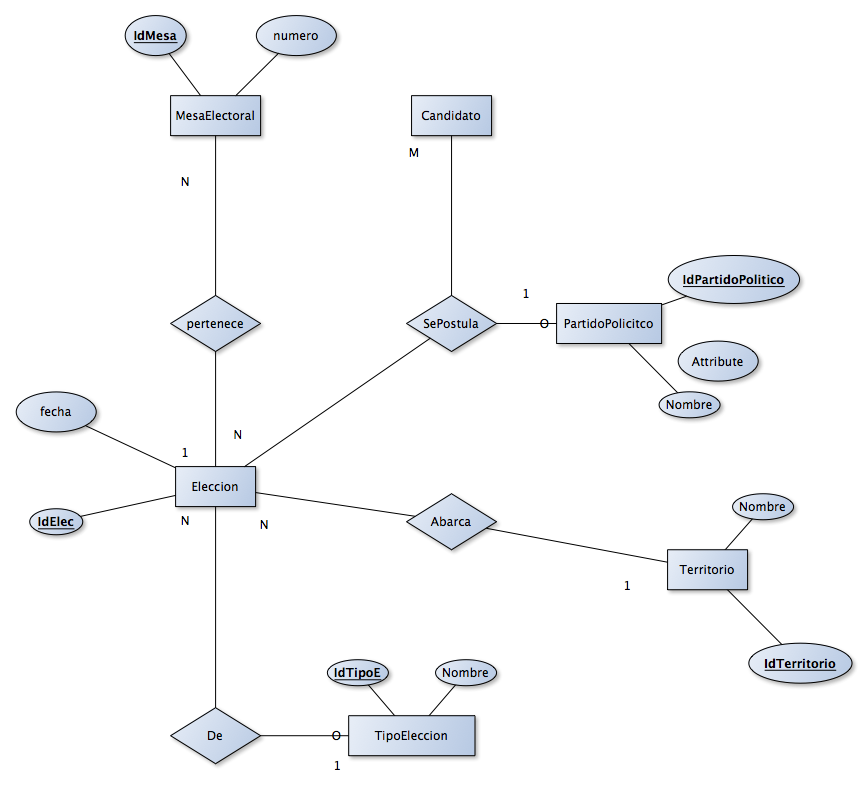
\includegraphics[scale=0.5]{graphics/der_eleccion.png}
   \caption{\textbf{Elecciones}}
   \label{fig:der}
   \end{center}
\end{figure}

Veamos finalmente cómo una Elección se modela dentro del sistema. Ésta se relaciona con las mesas electorales que le pertenecen, abarca un territorio y en ella se postulan candidatos de diferentes partidos políticos (cuando la elección es por un candidato y no un plebiscito).\\

El Tipo de Elección determina si es un plebiscito o no, y qué cargo se está eligiendo en caso de ser por un candidato. En esta implementación del sistema, esta distinción se realiza a través del atributo \textit{nombre} de TipoElección.\\

Consideramos que una mejor solución hubiera sido realizar una herencia disjunta de TipoElección a \textit{TipoElecciónCandidato} y \textit{TipoElecciónPlebiscito}, para poder modelar diferentes tipos de plebiscito (por ejemplo: legales, territoriales, emergencias, etc). No realizamos esta implementación por falta de tiempo.\\

A continuación presentamos el DER completo, que combina las diferentes partes vistas arribas.

\subsection{DER completo}
\begin{figure}[H]
   \begin{center}
   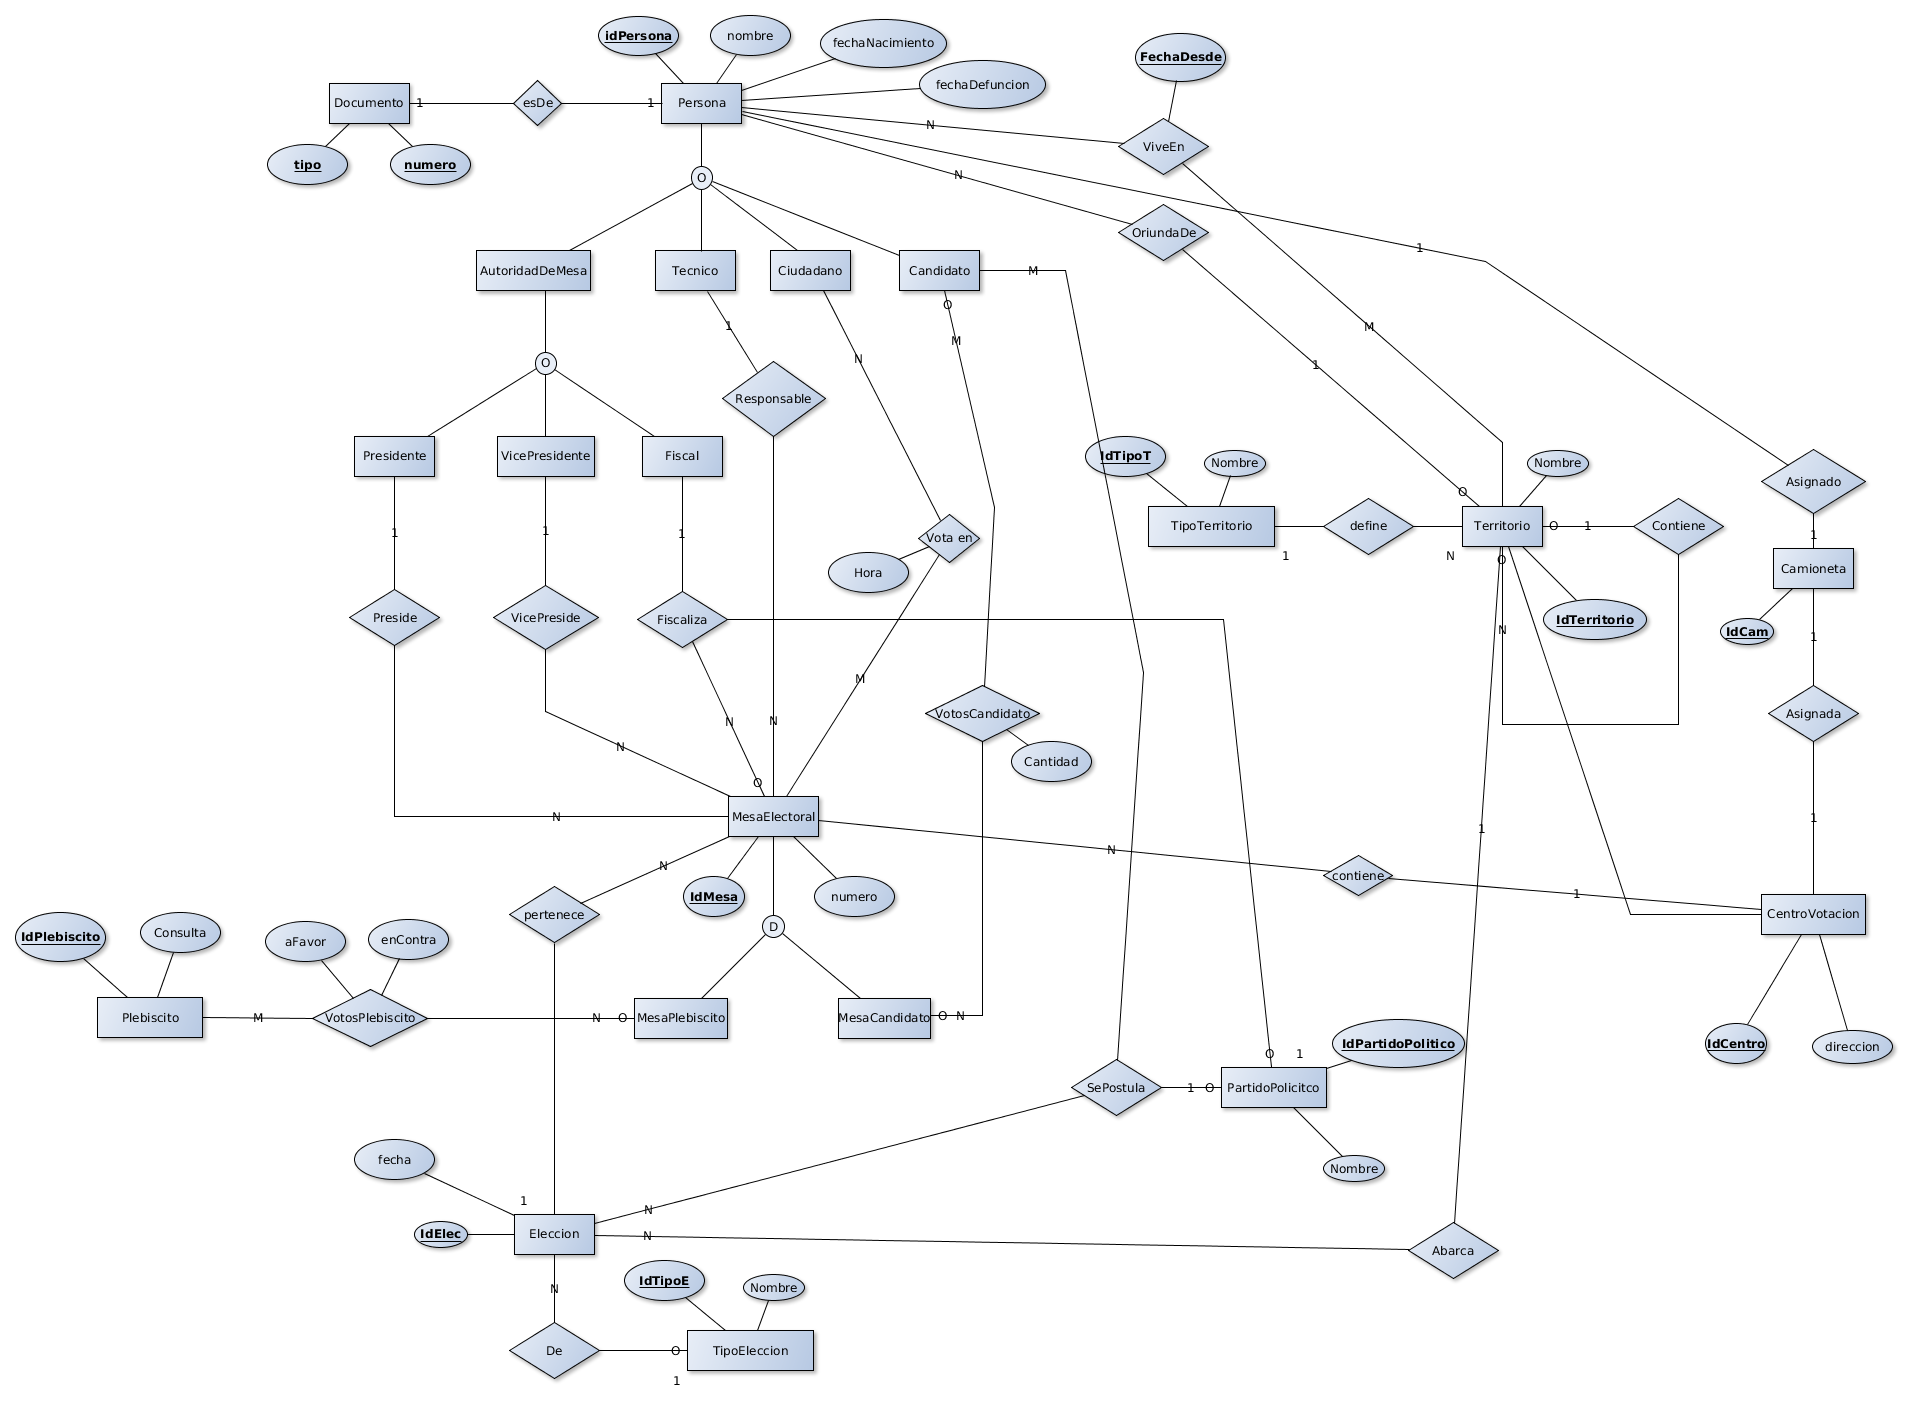
\includegraphics[angle=90,scale=0.32]{graphics/der.png}
   \caption{\textbf{Diagrama Entidad-Relación}}
   \label{fig:der}
   \end{center}
\end{figure}

\subsection{Restricciones Adicionales}

\subsubsection{Sobre los atributos}

\begin{itemize}
	\item{El número del Documento tiene que ser mayor a cero}.
	\item{El tipo del Documento tiene que ser alguno de los siguientes:
		\begin{itemize}
			\item{DNI}
			\item{CI}
			\item{LE}
			\item{LC}
		\end{itemize}
	}	
	\item{El atributo cantidad de la relación VotosCandidato tiene que ser mayor o igual a cero}

	\item{El atributo nombre de TipoTerritorio debe ser alguno de los siguientes y no se pueden repetir:
	  \begin{itemize}
	  	\item{País}
	  	\item{Provincia}
	  	\item{Localidad}
	  	\item{Ciudad}
	  \end{itemize}
	 }
	\item{El número de la MesaElectoral tiene que ser mayor a cero.}
	\item{Los  atributos aFavor y enContra de la relación VotosPlebiscito  tienen que ser mayor o igual a 0.}
	\item{El atributo fechaNacimiento no puede ser posterior al atributo fechaDefunción.}
\item{El atributo nombre de TipoEleccion debe ser alguno de los siguientes y no se pueden repetir:
	\begin{itemize}
		\item{Presidencial}
		\item{Gobernador}
		\item{Intendente}
		\item{Plebiscito}
	\end{itemize}
}

\item{Territorios sólo pueden contener a territorios más chicos:
\begin{itemize}
	\item{Un País sólo puede contener Provincias.}
	\item{Una Provincia sólo puede contener Localidades o Ciudades.}
	\item{Una Localidad sólo puede contener Ciudades.}
	\item{Una Ciudad no puede contener nada.}
\end{itemize}
}
\item{Sólo se puede ser oriundo de una ciudad.}

\item{El atributo fechaDesde de la relación ViveEn tiene que estar entre fechaNacimiento y fechaDefunción de la persona correspondiente.}

%Votar en las elecciones que corresponden según territorio.

\item{Para que un Ciudadano pueda participar en VotosCandidato o VotosPlebiscito con la MesaElectoral correspondiente, ésta debe pertenecer a una Eleccion que abarque un Territorio el cual debe ser igual o contiene en algún nivel al Territorio en el cual el Ciudadano ViveEn en el momento de la elección.\footnote{Quien participa de ViveEn es Persona, no Ciudadano. Nos estamos refiriendo a la Persona correspondiente a dicho Ciudadano.}
}

%Presentarse como candidato para la elección de algún cargo.

\item{Para que un Candidato pueda participar de SePostula con un PartidoPolítico en una Eleccion, el Territorio que esta última abarca debe ser igual o contener en algún nivel al Territorio en el cual el Candidato debe participar en ViveEn\footnote{Idem [1] pero para Candidato.} con una fechaDesde mayor a los X años.
}

%Solamente reciben votos los candidatos que se presentan a la elección.

\item{Para que un Candidatos puede participar de VotosCandidato con MesaCandidato, debe participar en SePostula con la Elección a la cual la MesaElectoral pertenece.
}

%Si el Partido Político tiene fiscales, tiene que postularse.

\item{Para que PartidoPolítico participe de fiscaliza con una MesaElectoral, debe participar en sePostula con un Candidato en una Elección que contenga esa MesaElectoral.}

\item{Dentro de una Elección, los números de MesaElectoral no se pueden repetir.}

\item{Para cada elección, una Persona sólo puede ser Presidente, VicePresidente, Fiscal, Candidato o Técnico de manera disjunta.}

\item{Los Ciudadanos solo pueden ser Autoridad de la Mesa en que votan}

\item{Ciudadanos sólo pueden votarEn una única MesaElectoral por Elección.}

\item{No puede pasar que para una elección haya por lo menos una  MesasElectorales y por lo menos una MesaPlebiscito.}

%No hay más votos que votantes

\item{Para cada MesaCandidato, la sumatoria de cantidad en cada tupla de VotoCandidato debe ser menor igual a la cantidad de tuplas en la relación VotaEn entre MesaElectoral y Ciudadano.}

\item{Para cada MesaPlebiscito, la sumatoria de aFavor y enContra en cada tupla de VotoPlebiscito debe ser menor igual a la cantidad de tuplas en la relación VotaEn entre MesaElectoral y Ciudadano.}

\item{Mayor de 16 para votar.}

\item{Para que una Persona sea Autoridad de Mesa tiene que tener más de 16 años.}

% Los muertos no votan

\item{Para que un Ciudadano participe en VotaEn con una MesaElectoral, no debe tener fecha de defunción anterior a la fecha de la Elección correspondiente a esa Mesa.}

\item{No puede haber 2 o más  elecciones con misma fecha y mismo TipoEleccion para mismo Terrritorio.}

\item{El CentroVotacion tiene q estar en un territorio contenido en el de la eleccion y que ademas sea una ciudad.}

\end{itemize}


\subsection{Consideraciones}

\subsubsection{Acerca de las afiliaciones a los partidos políticos}

\begin{itemize}
\item{Hemos decidido no modelar las afiliaciones de las personas a los partidos políticos, no sólo porque podrían ser muchas tuplas, sino que no nos parece un aspecto central del problema a modelar.}

\item{Consideramos que las afiliaciones a los partidos políticos de fiscales y candidatos se entienden por sus participaciones en fiscaliza y sePostula, respectivamente.}
\end{itemize}

\subsubsection{Sobre el impedimento para postularse según lugar de nacimiento.}

\begin{itemize}
\item{Sabemos que ciertos cargos requieren que un candidato haya nacido en el territorio correspondiente a la elección, como por ejemplo la elección de Presidente.Sin embargo, esto no es requerido para todos los cargos políticos y por ese motivo no forzamos esa restricción.}
\end{itemize}
